\experiment{Polynomial Addition}{27/09/2023}

\section{Aim}
Write a program to read two polynomials and store them in two arrays. Calculate the sum of
the two polynomials and display the first polynomial, second polynomial and the resultant
polynomial.

\section{Algorithm}
 {\fontfamily{lmtt}\selectfont

  \subsection{Structure Definition}
  Create a structure \texttt{Term} with the following attributes:
  \begin{enumerate}[label=\arabic*:,left=0pt]
    \item Integer \texttt{exp} to store the exponent of the term.
    \item Integer \texttt{coeff} to store the coefficient of the term.
  \end{enumerate}

  Create a structure \texttt{polynomial} with the following attributes:
  \begin{enumerate}[label=\arabic*:,left=0pt]
    \item Pointer to \texttt{Term} \texttt{terms} to store an array of terms.
    \item Integer \texttt{length} to store the number of terms in the polynomial.
    \item Integer \texttt{size} to store the maximum size of the polynomial.
  \end{enumerate}

  \subsection{Create Polynomial Function}
  Create a function \texttt{createPolynomial(size)}:
  \begin{enumerate}[label=\arabic*:,left=0pt]
    \item \textbf{Start}
    \item Allocate memory for a new \texttt{polynomial} structure using \texttt{malloc}.
    \item Allocate memory for the \texttt{terms} array using \texttt{malloc} with size \texttt{size}.
    \item Set \texttt{size} of the polynomial to \texttt{size}.
    \item Set \texttt{length} to 0.
    \item Return the created polynomial.
    \item \textbf{Stop}
  \end{enumerate}

  \subsection{Insert Term Function}
  Create a function \texttt{insertTerm(p, coeff, exp)}:
  \begin{enumerate}[label=\arabic*:,left=0pt]
    \item \textbf{Start}
    \item If \texttt{p->length} is equal to \texttt{p->size}, print "Polynomial size exceeded!" and return.
    \item Set \texttt{p->terms[p->length].coeff} to \texttt{coeff}.
    \item Set \texttt{p->terms[p->length].exp} to \texttt{exp}.
    \item Increment \texttt{p->length}.
    \item \textbf{Stop}
  \end{enumerate}

  \subsection{BubbleSort Function}
  Create a function \texttt{bubblesort(arr, size)}:
  \begin{enumerate}[label=\arabic*:,left=0pt]
    \item \textbf{Start}
    \item Loop from \texttt{i} equal to \texttt{size - 1} down to 0:
          \begin{enumerate}[label=2.\arabic*:, start=1]
            \item Loop from \texttt{j} equal to 0 to \texttt{i}:
                  \begin{enumerate}[label=2.1.\arabic*:, start=1]
                    \item If \texttt{arr[j].exp > arr[j + 1].exp}, swap \texttt{arr[j]} and \texttt{arr[j + 1]}.
                  \end{enumerate}
          \end{enumerate}
    \item \textbf{Stop}
  \end{enumerate}

  \subsection{Display Function}
  Create a function \texttt{display(p)}:
  \begin{enumerate}[label=\arabic*:,left=0pt]
    \item \textbf{Start}
    \item Loop from \texttt{i} equal to 0 to \texttt{p->length - 1}:
          \begin{enumerate}[label=2.\arabic*:, start=1]
            \item If \texttt{i} is not 0, print " + ".
            \item Print \texttt{p->terms[i].coeff} and \texttt{p->terms[i].exp}.
          \end{enumerate}
    \item Print a newline.
    \item \textbf{Stop}
  \end{enumerate}

  \subsection{Add Function}
  Create a function \texttt{add(p, q)}:
  \begin{enumerate}[label=\arabic*:,left=0pt]
    \item \textbf{Start}
    \item Set \texttt{result} to \texttt{createPolynomial(p->size + q->size)}.
    \item Set \texttt{i} and \texttt{j} to 0.
    \item Loop while \texttt{i < p->length || j < q->length}:
          \begin{enumerate}[label=2.\arabic*:, start=1]
            \item If \texttt{i >= p->length}, insert term with \texttt{q->terms[j].coeff} and \texttt{q->terms[j].exp} into \texttt{result}, \newline increment \texttt{j}, and continue to the next iteration.
            \item If \texttt{j >= q->length}, insert term with \texttt{p->terms[i].coeff} and \texttt{p->terms[i].exp} into \texttt{result}, \newline increment \texttt{i}, and continue to the next iteration.
            \item If \texttt{p->terms[i].exp < q->terms[j].exp}, insert term with \texttt{p->terms[i].coeff} and \newline \texttt{p->terms[i].exp} into \texttt{result} and increment \texttt{i}.
            \item If \texttt{p->terms[i].exp > q->terms[j].exp}, insert term with \texttt{q->terms[j].coeff} and \newline \texttt{q->terms[j].exp} into \texttt{result} and increment \texttt{j}.
            \item If \texttt{p->terms[i].exp = q->terms[j].exp}, insert term with \texttt{p->terms[i].coeff + \newline q->terms[j].coeff} and \texttt{p->terms[i].exp} into \texttt{result} and increment both \texttt{i} and \texttt{j}.
          \end{enumerate}
    \item Return \texttt{result}.
    \item \textbf{Stop}
  \end{enumerate}

  \subsection{Main Function}
  In the \texttt{main} function:
  \begin{enumerate}[label=\arabic*:, start=1]
    \item \textbf{Start}
    \item Declare \texttt{a} and \texttt{b} as \texttt{NULL}.
    \item Declare integers \texttt{n1} and \texttt{n2}.
    \item Print "Enter the number of terms of a: ".
    \item Take user input for \texttt{n1} and create a polynomial \texttt{a} using \texttt{createPolynomial(n1)}.
    \item Loop \texttt{n1} times and take user input for coefficients and exponents to insert terms into \texttt{a}.
    \item Print "Enter the number of terms of b: ".
    \item Take user input for \texttt{n2} and create a polynomial \texttt{b} using \texttt{createPolynomial(n2)}.
    \item Loop \texttt{n2} times and take user input for coefficients and exponents to insert terms into \texttt{b}.
    \item Call \texttt{bubblesort(a->terms, n1)} and \texttt{bubblesort(b->terms, n2)}.
    \item Print "a = " and call \texttt{display(a)}.
    \item Print "b = " and call \texttt{display(b)}.
    \item Call \texttt{add(a, b)} and assign the result to \texttt{sum}.
    \item Print "Sum = " and call \texttt{display(sum)}.
    \item Free memory allocated for \texttt{a}, \texttt{b}, and \texttt{sum}.
    \item \textbf{Stop}
  \end{enumerate}
  \textbf{End Algorithm}
 }

\section{C Program}
\begin{lstlisting}[label={list:c_program:polynomial_operations}]
#include <stdlib.h>
#include <stdio.h>

typedef struct Term
{
  int exp;
  int coeff;
} term;

typedef struct polynomial
{
  term *terms;
  int length;
  int size;
} polynomial;

polynomial *createPolynomial(int size);
void insertTerm(polynomial *p, int coeff, int exp);
void display(polynomial *p);
void bubblesort(term *arr, int size);
polynomial *add(polynomial *p, polynomial *q);

int main()
{
  polynomial *a = NULL;
  polynomial *b = NULL;
  int n1, n2;
  printf("Enter the number of terms of a: ");
  scanf("%d", &n1);
  a = createPolynomial(n1);
  for (int i = 0; i < n1; i++)
  {
    printf("\nEnter coefficient and exponents: ");
    int c, e;
    scanf("%d %d", &c, &e);
    insertTerm(a, c, e);
  }

  printf("\nEnter the number of terms of b: ");
  scanf("%d", &n2);
  b = createPolynomial(n2);
  for (int i = 0; i < n2; i++)
  {
    printf("\nEnter coefficient and exponents: ");
    int c, e;
    scanf("%d %d", &c, &e);
    insertTerm(b, c, e);
  }
  bubblesort(a->terms, n1);
  bubblesort(b->terms, n2);
  printf("a = ");
  display(a);
  printf("b = ");
  display(b);
  polynomial *sum = add(a, b);
  printf("Sum = ");
  display(sum);
  free(a);
  free(b);
  free(sum);
}

polynomial *createPolynomial(int size)
{
  polynomial *p = (polynomial *)malloc(sizeof(polynomial));
  p->terms = (term *)malloc(size * sizeof(term));
  p->size = size;
  p->length = 0;
  return p;
}

void insertTerm(polynomial *p, int coeff, int exp)
{
  if (p->length == p->size)
  {
    printf("\nPolynomial size exceeded!");
  }
  p->terms[p->length].coeff = coeff;
  p->terms[p->length].exp = exp;
  p->length++;
}

void bubblesort(term *arr, int size)
{
  for (int i = size - 1; i >= 0; i--)
  {
    for (int j = 0; j < i; j++)
    {
      if (arr[j].exp > arr[j + 1].exp)
      {
        int texp = arr[j].exp;
        int tcoeff = arr[j].coeff;
        arr[j].coeff = arr[j + 1].coeff;
        arr[j].exp = arr[j + 1].exp;
        arr[j + 1].coeff = tcoeff;
        arr[j + 1].exp = texp;
      }
    }
  }
}

void display(polynomial *p)
{
  for (int i = 0; i < p->length; i++)
  {
    if (i != 0)
      printf(" + ");
    printf("%dx^%d", p->terms[i].coeff, p->terms[i].exp);
  }
  printf("\n");
}

polynomial *add(polynomial *p, polynomial *q)
{
  term *result = createPolynomial(p->size + q->size);
  int i = 0, j = 0;
  while (i < p->length || j < q->length)
  {
    if (i >= p->length)
    {
      insertTerm(result, q->terms[j].coeff, q->terms[j].exp);
      j++;
      continue;
    }
    if (j >= q->length)
    {
      insertTerm(result, p->terms[i].coeff, p->terms[i].exp);
      i++;
      continue;
    }
    if (p->terms[i].exp < q->terms[j].exp)
    {
      insertTerm(result, p->terms[i].coeff, p->terms[i].exp);
      i++;
    }
    else if (p->terms[i].exp > q->terms[j].exp)
    {
      insertTerm(result, q->terms[j].coeff, q->terms[j].exp);
      j++;
    }
    else
    {
      insertTerm(result, p->terms[i].coeff + q->terms[j].coeff, p->terms[i].exp);
      i++;
      j++;
    }
  }
  return result;
}
\end{lstlisting}

\section{Output}
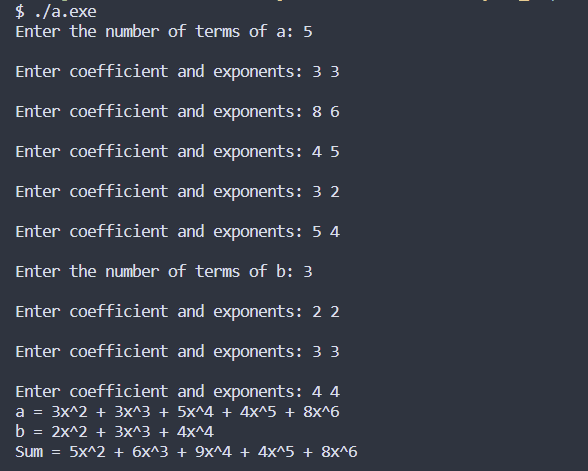
\includegraphics[]{Cycle_1/Outputs/Polynomial.png}

\section{Result}
Program to implement a program that performs addition on polynomials represented using arrays was implemented and its output was verified.